\section{Dicky Alfandra (1184019)}
\subsection{Teori}
\begin{enumerate}
\item Definisi Kecerdasan buatan\\ 
Dalam bidang komputer, Aritificial Intelligence (AI), atau biasa disebut juga sebagai Machine Intelligence merupakan bentuk dari representasi kecerdasan yang dilakukan oleh mesin, hampir mirip seperti bagaimana manusia melakukan kecerdasan. Beberapa sumber mendefinisikan  bahwa bidang yang mempelajari suatu agen kecerdasan merupakan suatu alat yang mengenali lingkungan sekitarnya dan mencoba untuk membuat kesimpulan untuk memaksimalkan kemungkinan tingkat keberhasilan dari pencapaian yang ingin dituju.

\item Sejarah dan Perkembangan Kecerdasan Buatan
\begin{itemize}
\item Pada tahun 1943, pekerjaan pertama yang dikenal sebagai AI telah dilakukan oleh Warren McCulloch dan juga Walter Pits yang dinamakan sebagai artificial neurons
\item Pada tahun 1955, Allen Newell dan Herbert A. Simon membuat program kecerdasan buatan pertama yang dinamakan Logic Theorist
\item Pada tahun 1972, robot pertama dibuat di jepang dengan nama Wabot-1 dengan kecerdasan buatan
\item Pada tahun 1980, muncul bidang baru dari kecerdasan buatan yaitu Expert System yang membantu dalam pemberian keputusan
\item Tahun 1997, IBM deep blue mengalahkan juara catur dunia Gary Kasparov dan menjadi komputer pertama yang mengalahkannya
\item Tahub 2006, perusahaaan sudah mulai menerapkan kecerdasan buatan pada produknya seperti Netflix dan Twitter.
\item Tahun 2018,  	Project Debater dari IBM melakuakn debat tentang topik yang kompleks dan berakhir dengan hasil memuaskan
\end{itemize}

\item Definisi Supervised Learning\\
Supervised Learning adalah proses untuk melatih mesin secara input dan output melalui contoh nyata secara langsung

\item Klasifikasi Supervised Learning
\begin{itemize}
\item Support Vector Machines
\item linear regression
\item logistic regression
\item naive Bayes
\item linear discriminant analysis
\item decision trees
\item k-nearest neighbor algorithm
\item Neural Networks (Multilayer perceptron)
\item Similarity learning
\end{itemize}

\item Regresi dan Unsupervised Learning\\
Regresi adalah suatu proses statistikal yang mengestimasi hubungan antara variable satu dengan variable yang lainnya.

Unsupervised Learning adalah bentuk dari machine learning yang mencari bentuk atau hubungan dari data set yang tidak mempunyai label dengan bantuan yang minimal dari manusia.

\item Dataset\\
Dataset adalah koleksi suatu data

\item Training Set\\
Training Set merupakan data yang digunakan untuk keperluan pembelajaran yang biasanya digunakan oleh machine learning

\item Testing Set\\
Testing set adalah data yang real yang digunakan untuk melatih machine learning

\end{enumerate}

\subsection{Instalasi}
\begin{enumerate}
	\item Instalasi Library scikit dari a naconda, mencoba kompilasi dan uji coba ambil contoh kode dan lihat variabel explorer
	\hfill\break
	\begin{figure}[H]
		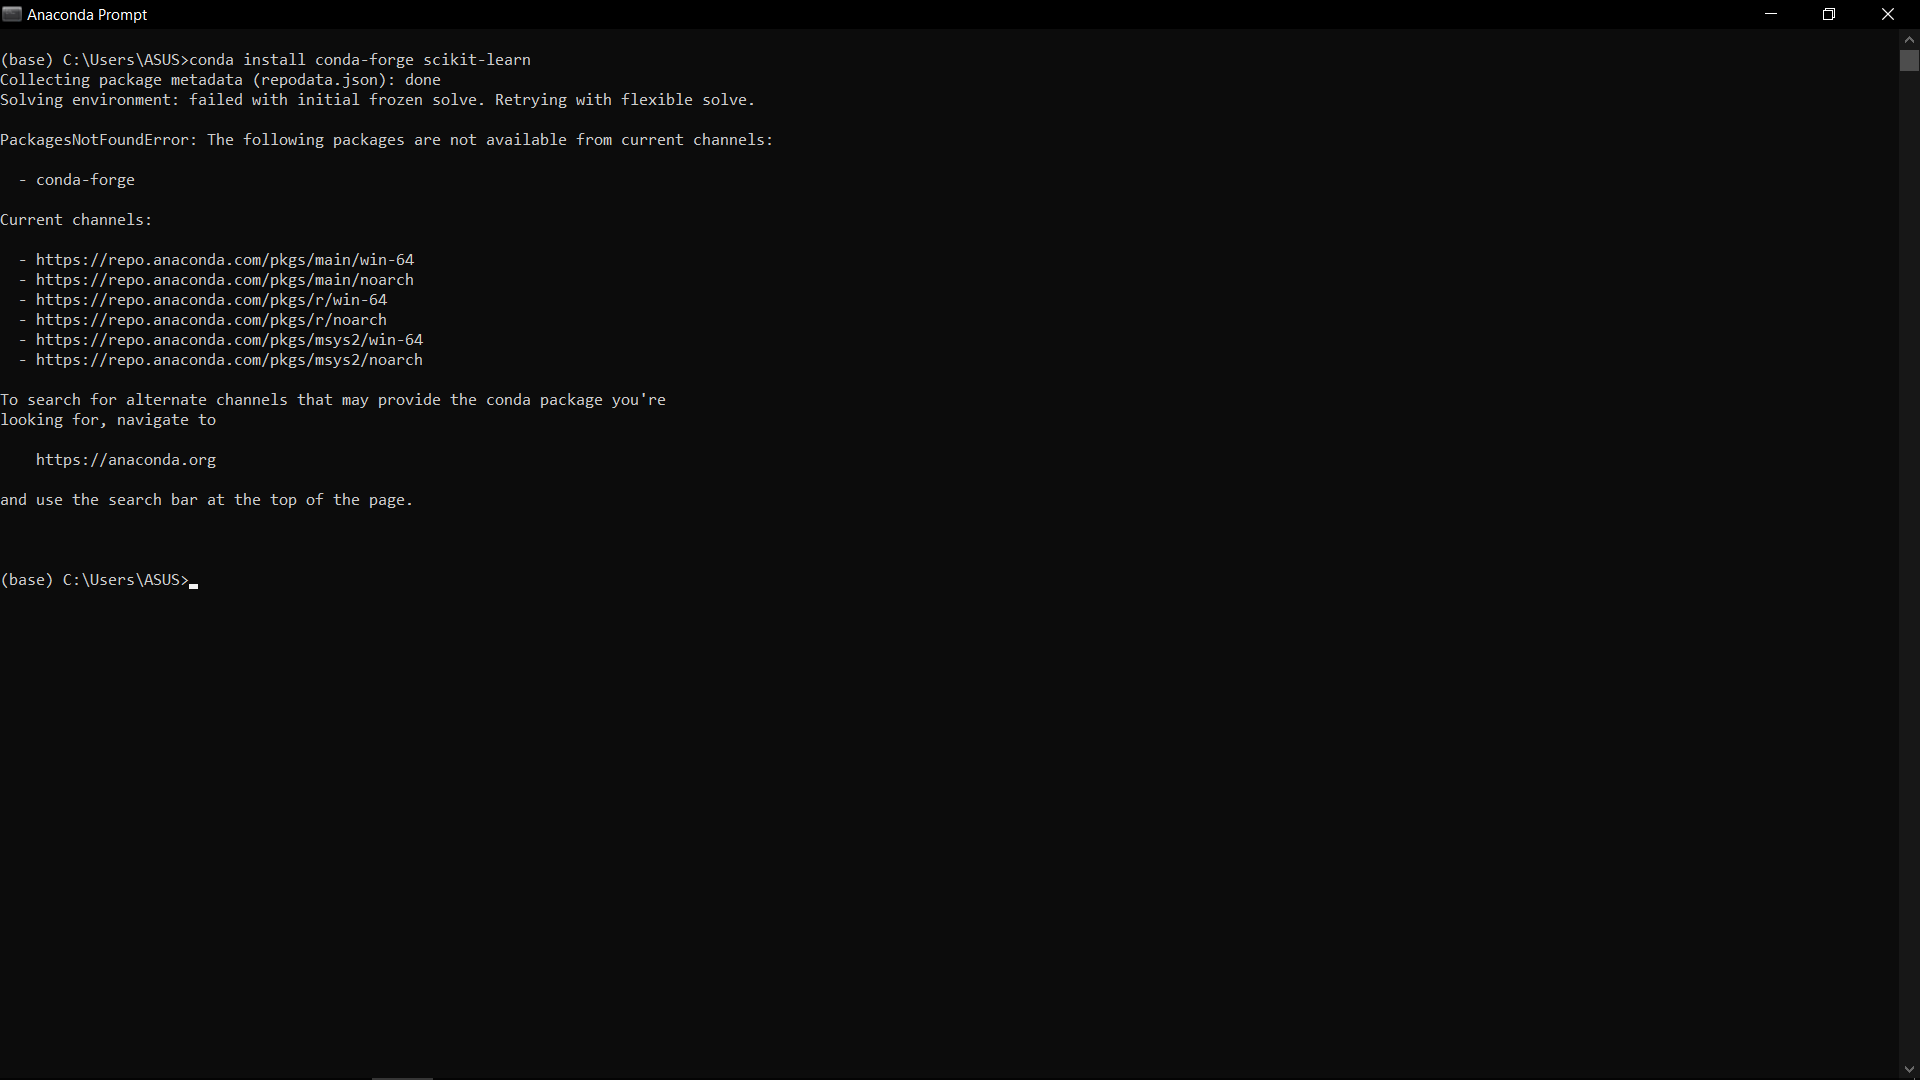
\includegraphics[width=4cm]{figures/1174079/1/1.png}
		\centering
		\caption{Instalasi Package Scikit Learn}
	\end{figure}
	\begin{figure}[H]
		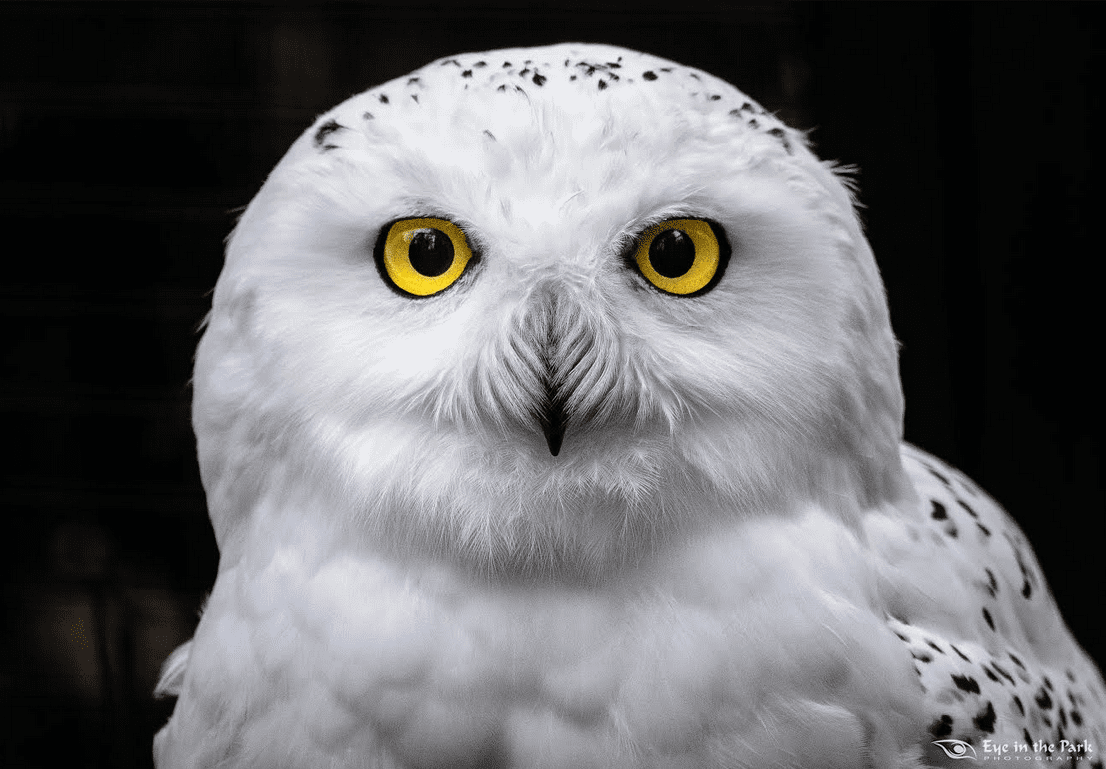
\includegraphics[width=4cm]{figures/1174079/1/2.png}
		\centering
		\caption{Isi Variabel Explorer}
	\end{figure}
	\item Mencoba Loading an example dataset, menjelaskan maksud dari tulisan tersebut dan mengartikan per baris
	\hfill\break
	\lstinputlisting[firstline=2, lastline=7]{src/1174079/1/1174079.py}
	\item Mencoba Learning and predicting, menjelaskan maksud dari tulisan tersebut dan mengartikan perbaris
	\hfill\break
	\lstinputlisting[firstline=9, lastline=28]{src/1174079/1/1174079.py}
	\item  Mencoba Model persistence, menjelaskan maksud dari tulisan tersebut dan mengartikan per baris
	\hfill\break
	\lstinputlisting[firstline=30, lastline=48]{src/1174079/1/1174079.py}
	\item Mencoba Conventions, menjelaskan maksud dari tulisan tersebut dan mengartikan per baris
	\hfill\break
	\lstinputlisting[firstline=50, lastline=72]{src/1174079/1/1174079.py}
\end{enumerate}

\subsection{Penanganan Error}
\begin{enumerate}
	\item ScreenShoot Error
	\begin{figure}[H]
		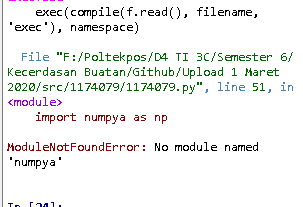
\includegraphics[width=4cm]{figures/1174079/1/error.PNG}
		\centering
		\caption{No Module Named Numpya}
	\end{figure}

	\item Tuliskan Kode Error dan Jenis Error
	\begin{itemize}
		\item ModuleNotFoundError
	\end{itemize}
	\item Cara Penangan Error
	\begin{itemize}
		\item ModuleNotFoundError
		\hfill\break
		Mengecek Typo dan menulis kembali library yang akan diimport
	\end{itemize}
\end{enumerate}

\subsection{Bukti Tidak Plagiat}
\begin{figure}[H]
	\includegraphics[width=4cm]{figures/1174079/1/plagiarism.PNG}
	\centering
	\caption{Bukti Tidak Melakukan Plagiat Chapter 1}
\end{figure}